\documentclass[tikz,border=2pt]{standalone}
\usepackage{pgfplots}
\usetikzlibrary{intersections}
\usepgfplotslibrary{fillbetween}
\pgfplotsset{compat=1.7}

\begin{document}
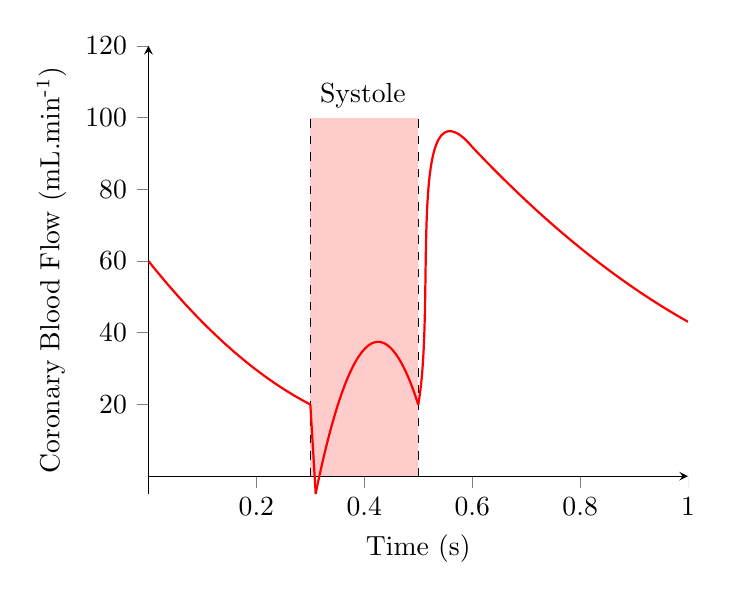
\begin{tikzpicture}


\begin{axis}[
        axis lines=middle,
        grid style={none},
	ymin = -5,
	ymax = 120,
	xmin = 0,
	xmax =1,
	 ylabel near ticks,
	xlabel near ticks,
        xlabel=Time (s),
        ylabel=Coronary Blood Flow (mL.min\textsuperscript{-1}),
        tick align=outside,
        enlargelimits=false,
legend pos= north west,
legend style={font=\small, cells={align=left}}]

\draw[name path=left, black, thin, dashed] (axis cs: 0.3,0) -- (axis cs: 0.3,100) node[pos=1, black, above right]{Systole};
\draw[name path=right, black, thin, dashed] (axis cs: 0.5,0) -- (axis cs: 0.5,100);
      \addplot[fill=red,opacity=0.2] fill between [of=left and right];
\plot[domain=0.6:1, red, thick,samples=500] {100 - 168.75*(x-0.55) + 93.75*(x-0.55)^2};
\plot[domain=0:0.3, red, thick,samples=500] {60 - 188.8889*x + 185.1852*x^2};
\draw[red, thick] (axis cs: 0.3, 20) -- (axis cs: 0.31, -5);
\plot[domain=0.31:0.5, red, thick,samples=500] {-534.8524 + 2689.709*x - 3160.254*x^2};
\draw[red, thick] (axis cs: 0.5,20) to[out=80,in=130] (axis cs: 0.6,91.8);


\end{axis}

\end{tikzpicture} 
\end{document}